% Copyright (C) 2022-2023 Florin-Ioan Subțirică


\documentclass{article}

\usepackage{float}
\usepackage{tabularx}
\usepackage{siunitx}
\usepackage[a4paper, total={6in, 8in}]{geometry}
\usepackage[utf8]{inputenc}
\usepackage[english, romanian]{babel}
\usepackage[hidelinks]{hyperref}
\usepackage{indentfirst}
\usepackage[siunitx, RPvoltages]{circuitikz}
\usepackage{fancyhdr}
\usepackage{xspace}
\usepackage{amssymb}
\usepackage{layout}
\usepackage{lastpage}
\usepackage{titling}
\usepackage{leftidx}
\usepackage{array}
\usepackage{enumitem}
\usepackage{titletoc,tocloft}
\usepackage{xcolor}
\usepackage{amsmath}
\usepackage{nicefrac}
\usepackage{mathtools}
\usepackage{graphicx}
\usepackage{multirow}


% Configuring the \latex command with sane defaults
\newcommand{\latex}{\LaTeX\xspace}

% Configuring the margins and layout
\oddsidemargin  = 13pt
\headheight     = 12pt
\textheight     = 674pt
\marginparsep   = 10pt
\footskip       = 30pt
\hoffset        = 0pt
\paperwidth     = 597pt
\topmargin      = -23pt
\headsep        = 25pt
\textwidth      = 426pt
\marginparwidth = 50pt
\marginparpush  = 5pt
\voffset        = 0pt
\paperheight    = 845pt

% Removing default header & footer configuration
\fancyhf{}

% Configuring the header
\pagestyle{fancy}
\lhead[Fizică]{Fizică}
\rhead[Florin-Ioan Subțirică]{Florin-Ioan Subțirică}

% Configuring the footer
\fancyhf[FR]{Pagina \thepage\ din \pageref{LastPage}}

% Setting up links inside content table
\hypersetup {
    citecolor = black,
    filecolor = black,
    linkcolor = black,
    urlcolor  = black,
    colorlinks,
}

% Configuring the titlepage
\title          {Difracția luminii printr-o fantă}
\author         {Florin-Ioan Subțirică \\ Seria CD, Grupa 322}
\date           {31.10.2022}
\predate{\centering}

\postdate{\vfill\emph{Facultatea de Automatică și Calculatoare}\hspace{2cm} \\
                \emph{Universitatea Politehnica București}     \hspace{2cm} \\
          \hfill\emph{2022 - 2023}\hfill}

% Configuring the table of contents
\setlength{\cftsubsecindent}{1cm}
\setlength{\cftsubsubsecindent}{2cm}
\dottedcontents{section}[1.5em]{}{1.3em}{.6em}



%%%%%%%%%%%%%%%%%%%%%%%%%%%%%%%%%%%%%%%%%%%%%%%%%%%%%%%%%%%%%%%%%%%%%%%%%%%%%%%


\begin{document}

% Project title
\maketitle
\thispagestyle{empty} % Remove page number
\pagebreak

% Table of contents
\tableofcontents
\thispagestyle{empty}
\pagebreak

% Introduction
\section        {Scopul lucrării}

\begin{enumerate}
    \item Se măsoară distribuția intensității luminoase difractate prin fante de lărgimi variabile.
    \item Se măsoară lungimea de undă a radiației difractate.
    \item Se verifică corespondența dintre teorie şi experiment în ceea ce priveştepoziţiile şi intensităţile maximelor de intensitate luminoasă.  
\end{enumerate}

\section        {Teoria lucrării}

\makebox[1cm]{} Difracţia reprezintă un ansamblu de fenomene specific undelor, care apare la
propagarea acestora într-un mediu cu neomogenităţi spaţiale pronunţate (de exemplu trecerea
lor prin fante transparente pentru unda studiată, practicate în ecrane opace, trecerea undei
lângă frontiera unui corp, etc). Fenomenul de difracţie este mai pronunţat când lungimea de
undă a undei este comparabilă cu dimensiunea obiectului difractant.

\makebox[1cm]{} Unda rezultată prin difracţie, este rezultatul interferenţei undelor difuzate de fiecare
punct al corpului difractant. Precizăm că dacă difracţia nu poate fi înţeleasă decât pe baza
interferenţei undelor difuzate, fenomenul de interferenţă poate fi însă explicat fără a face apel
la difracţie (de exemplu inelele lui Newton, interferometrul Fabry-Perot, etc).

\makebox[1.1cm]{} În studiul fenomenelor de difracţie, distingem două cazuri:
\begin{enumerate}
    \item Difracţie în lumină paralelă sau difracţie Fraunhofer, dacă direcţiile tuturor
    undelor care compun frontul de undă incident pe ecranul cu fantă sunt paralele; acesta
    corespunde unei distanţe infinite dintre sursa undelor şi ecran între ecran şi observator.
    Obţinerea luminii paralele se realizează fie cu un fascicul laser direct, fie cu un sistem de
    lentile (care transformă undele divergente din sursă, în unde plan paralele). 
    \item Difracţie în lumină convergentă sau difracţie Fresnel, când distanţele sus
    menţionate sunt finite. Acesta este cazul real întâlnit în practică, difracţia Fraunhofer fiind
    doar o aproximaţie care simplifică calculele. 
\end{enumerate}

\makebox[1cm]{} Să considerăm difracţia Fraunhofer a luminii provenită de la o sursă, printr-o fantă
transparentă plan paralelă de lărgime a, practicată în ecranul opac E (vezi fig.1.a). Razele
difractate sub unghiul $\varphi$ sunt forţate să interfereze cu ajutorul lentilei convergente L din fig
1.b. Imaginea reală de difracţie care apare pe ecranul E, aflat la distanţa D de fantă (vezi fig.
1.b) este prezentată în partea de jos a figurii 2. \newline
\makebox[1.5cm]{} Dacă lumina cade sub unghiul de incidenţă ${\varphi}{_0}$, atunci
intensitatea luminii difractate sub unghiul $\varphi$, este dată de: 

\begin{equation*}
    I = {I}{_0}\cdot\frac{Sin^2\epsilon}{\epsilon^2}
\end{equation*}

unde ${I}{_0}$ este intensitatea luminii incidente pe ecran în maximul central MC, iar mărimea $\epsilon$ este dată de:

\begin{equation*}
    \epsilon = \frac{\pi \cdot a}{\lambda} \cdot (sin(\varphi) - sin({\varphi}{_0}))
\end{equation*}

\begin{figure}[H]
    \centerline{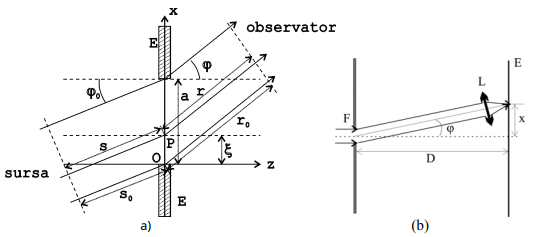
\includegraphics[scale = 0.7]{fig1.png}}
    \caption{a) Imaginea luminii difractate printr-o fantă plan paralelă b) Schema de
    \centerline{principiu a instalaţiei experimentale pentru studiul difracţiei printr-o fantă}}
    \label{}
\end{figure}

\begin{figure}[H]
    \centerline{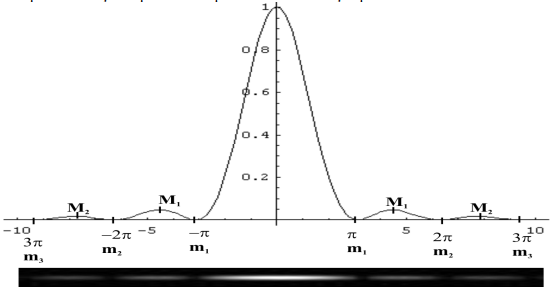
\includegraphics[scale = 0.7]{fig2.png}}
    \caption{Dependenţa imaginii difractate de poziţie, în planul ecranului E}
    \label{}
\end{figure}

\makebox[1cm]{} În figura 2 este prezentat dependenţa normata a intensităţii luminoase în funcţie de
parametrul adimensional $\epsilon$,

\begin{equation*}
    {I}{_n}(\epsilon) = \frac{I}{{I}{_0}} = \frac{Sin^2\epsilon}{\epsilon^2}
\end{equation*}

\makebox[1cm]{} Se observă că ea prezintă minime de intensitate (notate ${m}{_1}, {m}{_2}$,...) și maxime (notate
${M}{_1}, {M}{_2}$,...).

\section        {Dispozitivul experimental}

\makebox[1cm]{} Schema de principiu a instalaţiei folosite este prezentată în fig 3. Laserul L cu heliu-neon
fixat pe bancul optic gradat B emite lumină roşie cu puterea de circa 1 mW. Suportul S
permite fixarea diafragmei cu fante (cod 46991), prin intermediul a 2 cleme elastice.
Intensitatea luminii difractate este măsurată prin intermediul fotodiodei F şi a aparatului de
măsură A. Suportul fotodiodei este prevăzut cu o incintă protectoare care împiedică lumina
zilei să cadă pe fotodiodă şi să perturbe măsuratorile.

\begin{figure}[H]
    \centerline{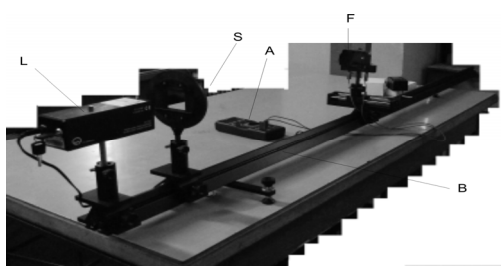
\includegraphics[scale = 0.7]{fig3.png}}
    \caption{Schema instalaţiei experimentale}
    \label{}
\end{figure}

\makebox[1cm]{} Această incintă este prevazută cu o fantă îngustă practicată în ecranul negru opac, care
permite măsurarea fluxului de lumină doar pe o zonă de lăgime
$\Delta x$ mică. Suportul S şi F pot
fi deplasate şi fixate pe bancul optic, respectiv pot fi deplasate pe verticală şi fixate prin
intermediul şuruburilor prezentate în fig. 4:

\begin{figure}[H]
    \centerline{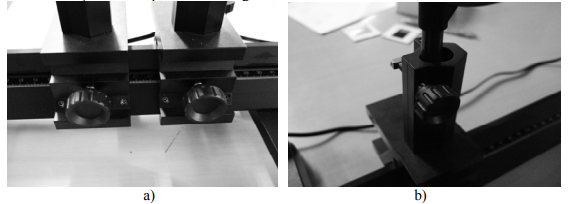
\includegraphics[scale = 0.7]{fig4.png}}
    \caption{a) şurub pentru fixarea componentelor instalaţiei pe bancul optic b) şurub pentru
    \centerline{fixare după ajustarea pe înălţime a componentelor instalaţiei}}
    \label{}
\end{figure}

\makebox[1cm]{} Distanţa x la care se măsoară intensitatea luminii difractate in planul ecranului E (care
coincide cu cel al fotodiodei F este măsurată pe rigla gradată din figura 5. Sistemul permite
deplasarea fotodiodei în direcţia riglei gradate prin rotaţia manetei din stânga figurii.

\begin{figure}[H]
    \centerline{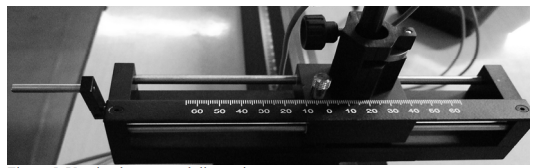
\includegraphics[scale = 0.7]{fig5.png}}
    \caption{Vernier de măsură al distanţei x}
    \label{}
\end{figure}

\section        {Modul de lucru}

\makebox[1cm]{} Înainte de pornirea circuitului ne-am asigurat că laserul este blocat astfel încât să nu se producă vreo catastrofă (leziuni ireversibile ale retinei ochiului). \newline
\makebox[1.53cm]{} Pentru pornirea lucrării am executat următorii pași: \newline
\newline
\makebox[1.53cm]{} 1. Am fixat laserul și am poziționat suportul S al diafragmei la circa 10 cm de capătul de ieșire al fascicolului laser.
După care am pus diafragma cu codul 46991 în suportul S cu ajutorul lamelelor elastice din suport. Diafragma are 3 fante diferite, acestea fiind prezentate în următorul tabel (Tabelul 1):

\begin{table}[H]
    \begin{tabular}{|l|l|l|l|}
    \hline
    Cod fantă          & A    & B    & C    \\ \hline
    Lărgime fantă (mm) & 0,12 & 0,24 & 0,48 \\ \hline
    \end{tabular}
    \end{table}

\makebox[1cm]{} 2. Am poziționat laserul întrucât lumina acestuia să cadă pe mijlocul diafragmei studiate (A sau B) și am pornit multimetrul pentru a măsura intensitatea luminii care cade pe fotodiodă, aproximată în funcție de tensiunea măsurată în mV. \newline
\makebox[1.5cm]{} 3. Am reglat și fixat poziția fotodiodei F pentru ca lumina laserului să cadă pe fanta verticală. \newline
\makebox[1.5cm]{} 4. Am rotit maneta atașată riglei fotodiodei, astfel încât vernierul s-a translatat pentru ca imaginea de difracție să cadă pe fanta fotodiodei. \newline
\makebox[1.5cm]{} 5. Am parcurs toată imaginea cu ajutorul vernierului și am notat pozițiile maxime și minime locale, ordinul acestora, cât și tensiunile aferente. \newline

\section        {Prelucrarea datelor experimentale}

\makebox[-0.7cm]{} Tabelul 2: Pozițiile minimelor de intensitate pentru fanta B

\begin{table}[H]
    \begin{tabular}{|cc|ccc|ccc|}
    \hline
    \multicolumn{2}{|c|}{Poziție față de MC}                                                                      & \multicolumn{3}{c|}{Stânga MC}                               & \multicolumn{3}{c|}{Dreapta MC}                         \\ \hline
    \multicolumn{2}{|c|}{Ordin minim}                                                                             & \multicolumn{1}{c|}{3}    & \multicolumn{1}{c|}{2}    & 1    & \multicolumn{1}{c|}{1}   & \multicolumn{1}{c|}{2} & 3   \\ \hline
    \multicolumn{1}{|c|}{\multirow{3}{*}{\begin{tabular}[c]{@{}c@{}}Poziție\\ X\\ riglă\end{tabular}}} & Măsur. 1 & \multicolumn{1}{c|}{-10}  & \multicolumn{1}{c|}{-6.5} & -3   & \multicolumn{1}{c|}{2.5} & \multicolumn{1}{c|}{6} & 9.5 \\ \cline{2-8} 
    \multicolumn{1}{|c|}{}                                                                             & Măsur. 2 & \multicolumn{1}{c|}{-9.5} & \multicolumn{1}{c|}{-6}   & -2.5 & \multicolumn{1}{c|}{3}   & \multicolumn{1}{c|}{6} & 9.5 \\ \cline{2-8} 
    \multicolumn{1}{|c|}{}                                                                             & Măsur. 3 & \multicolumn{1}{c|}{-10}  & \multicolumn{1}{c|}{-6.5} & -3   & \multicolumn{1}{c|}{2.5} & \multicolumn{1}{c|}{6} & 9.5 \\ \hline
    \end{tabular}
    \end{table}

\makebox[-0.7cm]{} Tabelul 3: Pozițiile și valorile maximelor de intensitate

\begin{table}[H]
    \begin{tabular}{|cc|ccc|c|ccc|}
    \hline
    \multicolumn{2}{|c|}{Poziție față de MC}                                                                  & \multicolumn{3}{c|}{Stânga MC}                               & \multirow{2}{*}{MC} & \multicolumn{3}{c|}{Dreapta MC}                              \\ \cline{1-5} \cline{7-9} 
    \multicolumn{2}{|c|}{Ordin minim}                                                                         & \multicolumn{1}{c|}{3}    & \multicolumn{1}{c|}{2}    & 1    &                     & \multicolumn{1}{c|}{1}    & \multicolumn{1}{c|}{2}    & 3    \\ \hline
    \multicolumn{1}{|c|}{\multirow{2}{*}{\begin{tabular}[c]{@{}c@{}}Fanta\\ B\end{tabular}}} & ${X}{_{maxim}}$  & \multicolumn{1}{c|}{3}    & \multicolumn{1}{c|}{6}    & 11   & 15,5                & \multicolumn{1}{c|}{20,5} & \multicolumn{1}{c|}{24}   & 27,5 \\ \cline{2-9} 
    \multicolumn{1}{|c|}{}                                                                   & ${U}{_F}$ (mV) & \multicolumn{1}{c|}{1,33} & \multicolumn{1}{c|}{3,27} & 6,41 & 104,3               & \multicolumn{1}{c|}{5.85} & \multicolumn{1}{c|}{1,77} & 0.84 \\ \hline
    \multicolumn{1}{|c|}{\multirow{2}{*}{\begin{tabular}[c]{@{}c@{}}Fanta\\ A\end{tabular}}} & ${X}{_{maxim}}$  & \multicolumn{1}{c|}{4}    & \multicolumn{1}{c|}{11}   & 22   & 34                  & \multicolumn{1}{c|}{42}   & \multicolumn{1}{c|}{54}   & 61   \\ \cline{2-9} 
    \multicolumn{1}{|c|}{}                                                                   & ${U}{_F}$ (mV) & \multicolumn{1}{c|}{0,73} & \multicolumn{1}{c|}{1,05} & 3,17 & 46,6                & \multicolumn{1}{c|}{1,96} & \multicolumn{1}{c|}{0,61} & 0,55 \\ \hline
    \end{tabular}
    \end{table}

\makebox[1cm]{} După completarea tabelelor de mai sus cu datele măsurate, începem să calculăm variabilele necesare pentru următorul tabel.

\makebox[1cm]{} Distanța medie ${X}{_{mn}}$ a minimului de ordin n se calculează cu relația:
\begin{equation*}
    {X}{_{mn}} = |\frac{{X}{_{sn}} - {X}{_{dn}}}{2}|
\end{equation*}
unde ${X}{_{sn}}$ și ${X}{_{dn}}$ reprezintă pozițiile citite pe rigla fotodiodei pentru minimele de ordin n, la stânga (${X}{_{sn}}$) și la dreapta (${X}{_{dn}}$) maximului central,
iar lungimea de undă se calculează cu
\begin{equation*}
    \lambda = \frac{{X}{_{mn}}\cdot a}{D\cdot n}
\end{equation*}
unde a este lățimea fantei, n este ordinul minim de intensitate, iar D este distanța dintre ecran și fantă. \newline

\makebox[-1cm]{} Tabelul 4: Determinarea lungimii de undă a laserului din poziţia minimelor de intensitate (Fanta B)

\begin{table}[H]
    \begin{tabular}{|c|ccc|ccc|ccc|}
    \hline
                      & \multicolumn{3}{c|}{Măsurătoarea 1}                          & \multicolumn{3}{c|}{Măsurătoarea 2}                         & \multicolumn{3}{c|}{Măsurătoarea 3}                          \\ \hline
    Ordin maxim       & \multicolumn{1}{c|}{1}    & \multicolumn{1}{c|}{2}    & 3    & \multicolumn{1}{c|}{1}    & \multicolumn{1}{c|}{2}    & 3   & \multicolumn{1}{c|}{1}    & \multicolumn{1}{c|}{2}    & 3    \\ \hline
    ${X}{_{mn}}$ (mm) & \multicolumn{1}{c|}{2.75} & \multicolumn{1}{c|}{6.25} & 9.75 & \multicolumn{1}{c|}{2.75} & \multicolumn{1}{c|}{6.00} & 9.5 & \multicolumn{1}{c|}{2.75} & \multicolumn{1}{c|}{6.25} & 9.75 \\ \hline
    $\lambda$ (nm)    & \multicolumn{1}{c|}{399}  & \multicolumn{1}{c|}{453}  & 471  & \multicolumn{1}{c|}{399}  & \multicolumn{1}{c|}{435}  & 459 & \multicolumn{1}{c|}{399}  & \multicolumn{1}{c|}{453}  & 471  \\ \hline
    \end{tabular}
    \end{table}

Cu cele 9 valori obținute, calculăm media și abaterea pătratică medie, prezentând rezultatele sub forma $\lambda = (\overline{\lambda} \pm {\sigma}{_{\lambda}})$ nm.

\begin{equation}
    \overline{\lambda} = \frac{\sum_{i=1}^{9}{\lambda}{_i}}{9} = 437.73 (nm)
\end{equation}

\begin{equation}
    {\sigma}{_{\lambda}} = \sqrt{\frac{\sum_{k=1}^{N}({\lambda}{_k} - \overline{\lambda})^2}{N(N-1)}} = 10.374 (nm)
\end{equation} \newline

Din (1) și (2) $\Rightarrow$ $\lambda$ = 437.73 $\pm$ 10.374 (nm) \newline

Folosind datele din tabelul 3, completăm tabelul 5. \newline

\makebox[-1cm]{} Tabelul 5: Comparația experiment-teorie pentru maximele de intensitate

\begin{table}[H]
    \begin{tabular}{|c|ccc|ccc|}
    \hline
                        & \multicolumn{3}{c|}{Fanta A}                                             & \multicolumn{3}{c|}{Fanta B}                                             \\ \hline
    Ordin maxim         & \multicolumn{1}{c|}{1}        & \multicolumn{1}{c|}{2}        & 3        & \multicolumn{1}{c|}{1}        & \multicolumn{1}{c|}{2}        & 3        \\ \hline
    ${X}{_{Mn e}}$ (mm) & \multicolumn{1}{c|}{10.00}    & \multicolumn{1}{c|}{21.50}    & 28.50    & \multicolumn{1}{c|}{4.75}     & \multicolumn{1}{c|}{9.00}     & 12.25    \\ \hline
    ${X}{_{Mn t}}$ (mm) & \multicolumn{1}{c|}{8.8386}   & \multicolumn{1}{c|}{15.1965}  & 21.4502  & \multicolumn{1}{c|}{4.4193}   & \multicolumn{1}{c|}{7.5983}   & 10.7251  \\ \hline
    ${k}{_{xM}}$        & \multicolumn{1}{c|}{1.1314}   & \multicolumn{1}{c|}{1.4148}   & 1.3287   & \multicolumn{1}{c|}{1.0748}   & \multicolumn{1}{c|}{1.1845}   & 1.1422   \\ \hline
    ${I}{_{ne}}$        & \multicolumn{1}{c|}{0.068026} & \multicolumn{1}{c|}{0.022532} & 0.015665 & \multicolumn{1}{c|}{0.061398} & \multicolumn{1}{c|}{0.031322} & 0.012739 \\ \hline
    ${k}{_I}$           & \multicolumn{1}{c|}{1.4412}   & \multicolumn{1}{c|}{1.3412}   & 1.8783   & \multicolumn{1}{c|}{1.3008}   & \multicolumn{1}{c|}{1.8644}   & 1.5275   \\ \hline
    \end{tabular}
    \end{table}

\begin{equation*}
    {X}{_{Mn e}} = |\frac{{X}{_{sn}} - {X}{_{dn}}}{2}|
\end{equation*}

unde ${X}{_{sn}}$ și ${X}{_{dn}}$ reprezintă pozițiile maxime de ordin n

\begin{equation*}
    {X}{_{Mn t}} = \frac{\lambda D {\epsilon}{_M}}{\pi a}
\end{equation*}

\makebox[-0.7cm]{} unde $\lambda$ e cea obținută puțin mai sus, iar parametrii a și $\epsilon$ sunt extrași din tabelul 1, respectiv [A1] \newline

\makebox[-0.7cm]{} Tabelul A1:
\begin{table}[H]
    \begin{tabular}{|c|c|c|c|}
    \hline
    Ordin maxim                       & 1      & 2      & 3       \\ \hline
    ${\epsilon}{_M}$ = poziție maximă & 4,493  & 7,725  & 10,904  \\ \hline
    ${I}{_n}(\epsilon)$               & 0,0472 & 0,0168 & 0,00834 \\ \hline
    \end{tabular}
    \end{table}

Parametrul ${k}{_{xM}}$ este definit prin:

\begin{equation*}
    {k}{_{xM}} = \frac{{X}{_{Mn e}}}{{X}{_{Mn t}}}
\end{equation*}

\begin{equation}
    \overline{{k}{_{xM}}} = \frac{\sum_{i=1}^{6}{{k}{_{xM}}}{_i}}{6} = 1.2127
\end{equation}

\begin{equation}
    {\sigma}{_{{k}{_{xM}}}} = \sqrt{\frac{\sum_{k=1}^{N}({{k}{_{xM}}}{_k} - \overline{{k}{_{xM}}})^2}{N(N-1)}} = 0.053440
\end{equation} \newline

Din (3) și (4) $\Rightarrow$ ${k}{_{xM}}$ = 1.2127 $\pm$ 0.053440 \newline

El reprezintă o evaluare a acurateţii teoriei, fiind la modul ideal egal cu unitatea. \newline \newline

Parametrul ${I}{_{ne}}$ este definit prin:

\begin{equation*}
    {I}{_{ne}} = \frac{{I}{_k}}{{I}{_0}}
\end{equation*}

unde ${I}{_k}$ este (pentru o fantă dată) intensitatea maximului de ordin k, iar ${I}{_0}$ intensitatea maximului central. \newline \newline 

Comparația teorie-experiment se face prin intermediul parametrului ${k}{_I}$ definit prin:

\begin{equation*}
    {k}{_I} = \frac{{I}{_{ne}}}{{I}{_{nt}}}
\end{equation*}

unde predicția teoretică ${I}{_{nt}}$ a intensității normate este oferită de ultima linie a tabelului A1. 

\begin{equation}
    \overline{{k}{_I}} = \frac{\sum_{i=1}^{6}{{k}{_I}}{_i}}{6} = 1.5589
\end{equation}

\begin{equation}
    {\sigma}{_{{k}{_I}}} = \sqrt{\frac{\sum_{k=1}^{N}({{k}{_I}}{_k} - \overline{{k}{_I}})^2}{N(N-1)}} = 0.1040
\end{equation} \newline

Din (5) și (6) $\Rightarrow$ $\lambda$ = 1.5589 $\pm$ 0.1040 \newline

\section{Anexă}
\space\space\space\space \href{https://ctipub-my.sharepoint.com/:f:/g/personal/florin_subtirica_stud_acs_upb_ro/Eq0TbKFmnjhAoszjx_vnN18Bn3oi9FP3BmvfzAQFApd__Q?e=SbfAlY}{Referat} \newline

\begin{thebibliography}{10}

    $\href{http://www.physics.pub.ro/Referate/BN031A/Difractia_luminii_printr-o_fanta_+_Relatiile_de_incertitudine_ale_lui_HEISENBERG.pdf}{Teorie}$

\end{thebibliography}
        
    \addcontentsline{toc}{section}{Bibliografie}

\end{document}

%%%%%%%%%%%%%%%%%%%%%%%%%%%%%%%%%%%%%%%%%%%%%%%%%%%%%%%%%%%%%%%%%%%%%%%%%%%%%%%